\documentclass{math}

\usepackage{pgfplots}
\usepackage{tikz}
\usepgfplotslibrary{fillbetween}
\usetikzlibrary{patterns}

\geometry{letterpaper, margin=0.5in}

\title{Multivariable and Vector Calculus: Homework 7}
\author{Alvin Lin}
\date{August 2016 - December 2016}

\begin{document}

\maketitle

\section*{Section 14.7}

\subsubsection*{Exercise 9}
Find the local maximum and minimum values and saddle point(s) of the function.
\[ f(x,y) = x^2+y^4+2xy \]
\begin{align*}
  f_x &= 2x+2y \\
  f_y &= 4y^3+2x \\
  f_x &= 0 = 2x+2y \\
  x &= -y \\
  f_y &= 4y^3+2x = 0 \\
  &\equiv 4(-x)^3+2x = 0 \\
  0 &= -4x^3+2x \\
  0 &= x(-2x^2+1) \\
  x &= 0 \quad x = \pm\frac{1}{\sqrt{2}} \\
\end{align*}
Points of interest: \( (0,0), (-\frac{1}{\sqrt{2}},\frac{1}{\sqrt{2}}),
(\frac{1}{\sqrt{2}},-\frac{1}{\sqrt{2}}) \)
\begin{align*}
  f_{xx} &= 2 \\
  f_{xy} &= 2 \\
  f_{yy} &= 12y^2 \\
  D(0,0) &= 2(0)-4 = -4 \quad \text{Saddle Point}\\
  f(0,0) &= 0 \\
  D(-\frac{1}{\sqrt{2}},\frac{1}{\sqrt{2}}) &= 2(6)-4 = 8
    \quad \text{Relative Minimum}\\
  f(-\frac{1}{\sqrt{2}},\frac{1}{\sqrt{2}}) &= \frac{1}{2}+\frac{1}{4}-1 =
    -\frac{1}{4} \\
  D(\frac{1}{\sqrt{2}},-\frac{1}{\sqrt{2}}) &= 2(6)-4 = 8
    \quad \text{Relative Minimum} \\
  f(\frac{1}{\sqrt{2}},-\frac{1}{\sqrt{2}}) &= -\frac{1}{4}
\end{align*}

\subsubsection*{Exercise 17}
\[ f(x,y) = xy+\e^{-xy} \]
\begin{align*}
  f_x &= y-y\e^{xy} \\
  f_y &= x-x\e^{xy} \\
  f_x &= 0 = y-y\e^{xy} \\
  0 &= y(1-\e^{xy}) \\
  \e^{xy} &= 1 \\
  xy &= 0 \\
  y &= 0 \text{ or } x = 0 \\
\end{align*}
Points of interest: \( (0,y), (x,0) \)
\begin{align*}
  f_{xx} &= y^2\e^{xy} \\
  f_{xy} &= 1+xy\e^{-xy}-\e^{-xy} \\
  f_{yy} &= x^2\e^{-xy} \\
  D(0,y) &= D(x,0) = 0
\end{align*}
Inconclusive. By inspection of graph, \( (0,y), (x,0) \text{ are local
minima }\forall x,y \).
\[ f(0,y) = 1 \quad f(x,0) = 1 \]

\subsubsection*{Exercise 35}
Find the absolute maximum or minimum values of \( f \) on the set \( D \).
\[ f(x,y) = x^2+2y^2-2x-4y+1 \quad D = \{(x,y)\mid0\le x\le2,0\le y\le 3\} \]
\begin{align*}
  f_x &= 2x-2 \\
  f_y &= 4y-4 \\
  f_x &= 0 = 2x-2 \\
  x &= 1 \\
  f_y &= 0 = 4y-4 \\
  y &= 1
\end{align*}
Points of interest: \( (1,1), (x,0), (x,3), (0,y), (2,y) \)
\begin{itemize}
  \item \( (0,0) \)
  \[ f(1,1) = -2 \]
  \item \( (x,0) \)
  \begin{align*}
    f(x,0) &= x^2-2x+1 \\
    f_x &= 2x-2 = 0 \\
    x &= 1 \\
    f(1,0) &= 0 \quad f(0,0) = 1 \quad f(2,0) = 1
  \end{align*}
  \item \( (x,3) \)
  \begin{align*}
    f(x,3) &= x^2+18-2x-12+1 \\
    f_x &= 2x-2 = 0 \\
    x &= 1 \\
    f(1,3) &= 0 \quad f(0,3) = 7 \quad f(2,3) = 7
  \end{align*}
  \item \( (0,y) \)
  \begin{align*}
    f(0,y) &= 2y^2-4y+1 \\
    f_y &= 4y-4 = 0 \\
    y &= 1 \\
    f(0,1) &= -1 \quad f(0,0) = 1 \quad f(0,3) = 7
  \end{align*}
  \item \( (2,y) \)
  \begin{align*}
    f(2,y) &= 4+2y^2-4-4y+1 \\
    f_y &= 4y-4 = 0 \\
    y &= 1 \\
    f(2,1) &= -1 \quad f(2,0) = 1 \quad f(2,3) = 7
  \end{align*}
\end{itemize}
Absolute Minimum: -2 at (1,1) \\
Absolute Maximum: 7 at (2,3), and (0,3)

\subsubsection*{Exercise 47}
Find the maximum volume of a rectangular box that is inscribed in a sphere of
radius \( r \).
\begin{align*}
  \sqrt{l^2+w^2+h^2} &= 2r \\
  l^2+w^2+h^2 &= 4r^2 \\
  h &= \sqrt{4r^2-l^2-w^2} \\
  V &= lwh \\
  V(l,w) &= lw\sqrt{4t^2-l^2-w^2} \\
  V_l &= w\sqrt{4t^2-l^2-w^2}-\frac{l^2w}{\sqrt{4t^2-l^2-w^2}} \\
  0 &= w\sqrt{4t^2-l^2-w^2}-\frac{l^2w}{\sqrt{4t^2-l^2-w^2}} \\
  &= \frac{4t^2w-l^2w-w^3}{\sqrt{4t^2-l^2-w^2}}-
    \frac{l^2w}{\sqrt{4t^2-l^2-w^2}} \\
  &= w(4t^2-2l^2-w^2) \\
\end{align*}
\begin{align*}
  w &= 0 \quad w = \pm\sqrt{4t^2-2l^2} \\
  V_w &= l\sqrt{4t^2-l^2-w^2}-\frac{lw^2}{\sqrt{4t^2-l^2-w^2}} \\
  0 &= \frac{4t^2l-l^3-w^2l}{\sqrt{4t^2-l^2-w^2}}
    -\frac{lw^2}{\sqrt{4t^2-l^2-w^2}} \\
  &= l(4t^2-l^2-2w^2) \\
  &= 4t^2-l^2-2(4t^2-2l^2) \\
  &= 4t^2-l^2-8t^2+4l^2 \\
  4t^2 &= 3l^2 \\
  l &= \sqrt{\frac{4t^2}{3}} = \frac{2r}{\sqrt{3}} \\
  w &= \frac{2r}{\sqrt{3}} \\
  h &= \frac{2r}{\sqrt{3}} \\
  \text{maximum volume} &= lwh = \frac{8r^3}{3\sqrt{3}}
\end{align*}

\subsubsection*{Exercise 53}
A cardboard box without a lid is to have a volume of 32,000 \( \text{cm}^3 \).
Find the dimensions that minimize the amount of cardboard used.
\begin{align*}
  V &= lwh = 32000 \\
  h &= \frac{32000}{lw} \\
  SA &= 2wh+2lh+lw \\
  &= 2w\frac{32000}{lw}+2l\frac{32000}{lw}+lw \\
  &= \frac{64000}{l}+\frac{64000}{w}+lw \\
  SA_l &= -\frac{64000}{l^2}+w = 0 \\
  w &= \frac{64000}{l^2} \\
  SA_w &= -\frac{64000}{w^2}+l = 0 \\
  l &= \frac{64000}{w^2} \\
  l &= 64000\frac{l^4}{64000^2} \\
  l^3 &= 64000 \\
  l &= 40 \\
  w &= 40 \\
  h &= \frac{32000}{40^2} = 20
\end{align*}

\section*{Section 15.1}

\subsubsection*{Exercise 1}
Estimate the volume of the solid that lies below the surface \( z = xy \) and
above the rectangle
\[ R = \{(x,y)\mid0\le x\le6,0\le y\le4\} \]
Use a Riemann sum with \( m = 3, n = 2 \) and take the sample point to be the
upper right corner of each square.
\begin{align*}
  V &= 4f(2,2)+4f(4,2)+4f(6,2)+4f(4,2)+4f(4,4)+4f(4,6) \\
  &= 4(4+8+12+8+16+24) \\
  &= 16+32+48+32+64+96 \\
  &= 48+80+160 \\
  &= 288
\end{align*}

\section*{Section 15.2}

\subsubsection*{Exercise 9}
Evaluate the double integral.
\[ \iint_{D}\frac{y}{x^2+1}\diff{A} \quad
    D = \{(x,y)\mid0\le x\le4,0\le y\le\sqrt{x}\} \]
\begin{align*}
  \int_{0}^{4}\int_{0}^{\sqrt{x}}\frac{y}{x^2+1}\diff{y}\diff{x}
    &= \int_{0}^{4}\bigg[\frac{y^2}{2x^2+2}\bigg]_{0}^{\sqrt{x}}\diff{x} \\
  &= \frac{1}{2}\int_{0}^{4}\frac{x}{x^2+1}\diff{x} \\
  u &= x^2+1 \\
  \diff{u} &= 2x\diff{x} \\
  &= \frac{1}{2}\int_{0}^{4^2+1}\frac{x}{u}\frac{\diff{u}}{2x} \\
  &= \frac{1}{2}\int_{0}^{17}\frac{1}{2u}\diff{u} \\
  &= \frac{1}{4}\bigg[\ln(u)\bigg]_0^{17} \\
  &= \frac{1}{4}(\ln(17)-\ln(1)) \\
  &= \frac{\ln(17)}{4}
\end{align*}

\subsubsection*{Exercise 19}
Evaluate the double integral.
\[ \iint_{D}y^2\diff{A} \quad D \text{ is the triangular region with vertices }
  (0,1), (1,2), (4,1) \]
\begin{center}
  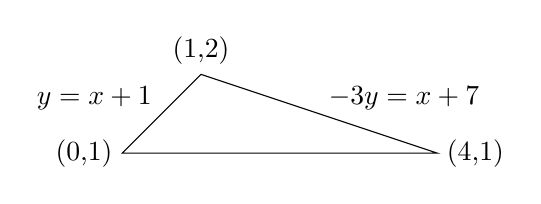
\begin{tikzpicture}
    \draw (0,1) node[left] {(0,1)} --
      node[pos=0.5,left,yshift=0.2cm] {\( y = x+1 \)} (1,2)
      node[above] {(1,2)} --
      node[pos=0.5,right,yshift=0.2cm] {\( -3y = x+7 \)} (4,1)
      node[right] {(4,1)} -- cycle;
  \end{tikzpicture}
\end{center}
\begin{align*}
  \int_{1}^{2}\int_{y-1}^{7-3y}y^2\diff{x}\diff{y} &=
    \int_{1}^{2}y^2\bigg[x\bigg]_{y-1}^{7-3y}\diff{y} \\
  &= \int_{1}^{2}y^2(7-3y-(y-1))\diff{y} \\
  &= \int_{1}^{2}8y^2-4y^3\diff{y} \\
  &= \bigg[\frac{8y^3}{3}-\frac{4y^4}{4}\bigg]_{1}^{2} \\
  &= \frac{8(8)}{3}-16-(\frac{8}{3}-1) \\
  &= \frac{64}{3}-\frac{48}{3}-\frac{8}{3}+\frac{3}{3} \\
  &= \frac{11}{3}
\end{align*}

\subsubsection*{Exercise 23}
Find the volume of the solid under the plane \( 3x+2y-z = 0 \) and above the
region enclosed by the parabolas \( y = x^2 \) and \( x = y^2 \).
\begin{align*}
  x &= 3x+2y \\
  \int_{0}^{1}\int_{x^2}^{\sqrt{x}}3x+2y\diff{y}\diff{x} &=
    \int_{0}^{1}\bigg[3xy+\frac{2y^2}{2}\bigg]_{x^2}^{\sqrt{x}} \\
  &= \int_{0}^{1}3x^{\frac{3}{2}}+x-(3x^3+x^4)\diff{x} \\
  &= \int_{0}^{1}3x^{\frac{3}{2}}-x^4-3x^3+x\diff{x} \\
  &= \bigg[
    \frac{6}{5}x^{\frac{5}{2}}-\frac{x^5}{5}-\frac{3x^4}{4}+\frac{x^2}{2}
    \bigg]_{0}^{1} \\
  &= \frac{6}{5}-\frac{1}{5}-\frac{3}{4}+\frac{1}{2}-(0) \\
  &= 1-\frac{3}{4}+\frac{1}{2} \\
  &= \frac{3}{4}
\end{align*}

\subsubsection*{Exercise 29}
Find the volume of the solid enclosed by the cylinders \( z = x^2, y = x^2 \)
and the planes \( z = 0, y = 4 \).
\begin{align*}
  \int_{-2}^{2}\int_{x^2}^{4}x^2\diff{y}\diff{x} &=
    2\int_{0}^{2}\int_{x^2}^{4}x^2\diff{y}\diff{x} \\
  &= 2\int_{0}^{2}x^2\bigg[y\bigg]_{x^2}^{4}\diff{x} \\
  &= 2\int_{0}^{2}x^2(4-x^2)\diff{x} \\
  &= 2\bigg[\frac{4x^3}{3}-\frac{x^5}{5}\bigg]_{0}^{2} \\
  &= 2(\frac{32}{3}-\frac{32}{5}-(0)) \\
  &= 2(\frac{160}{3}-\frac{96}{15}) \\
  &= 2(\frac{64}{15}) \\
  &= \frac{128}{15}
\end{align*}

\subsubsection*{Exercise 47}
Sketch the region of integration and change the order of integration.
\[ \int_{0}^{\frac{\pi}{2}}\int_{0}^{\cos(x)}f(x,y)\diff{y}\diff{x} \]
\begin{center}
  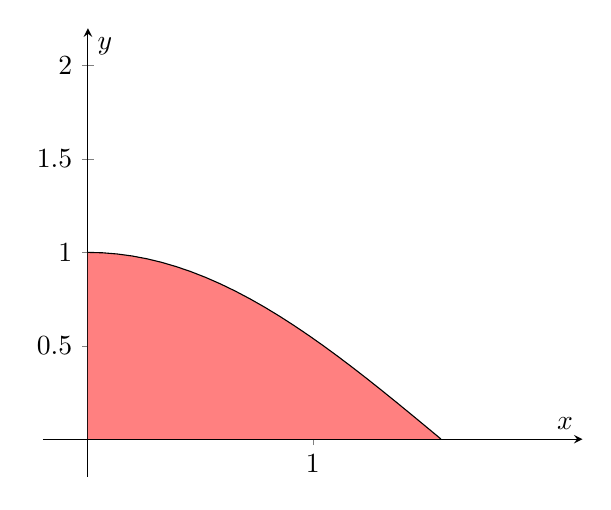
\begin{tikzpicture}
    \begin{axis}[axis lines=middle,
                 xlabel=\(x\), ylabel=\(y\),
                 ymin=0, ymax=2,
                 xmin=0, xmax=2,
                 enlargelimits,
                 xtick={0,1}]
      \addplot[name path=F, domain={0:1.57}]{cos(deg(x))};
      \addplot[name path=G, domain={0:1.57}]{0};
      \addplot[color=red!50] fill between [
               of=F and G, soft clip={domain=0:1.57}];
    \end{axis}
  \end{tikzpicture}
\end{center}
\[ \int_{0}^{1}\int_{0}^{\arccos(y)}f(x,y)\diff{x}\diff{y} \]

\subsubsection*{Exercise 51}
Evaluate the integral by reversing the order of integration.
\[ \int_{0}^{1}\int_{3y}^{3}\e^{x^2}\diff{x}\diff{y} \]
\begin{center}
  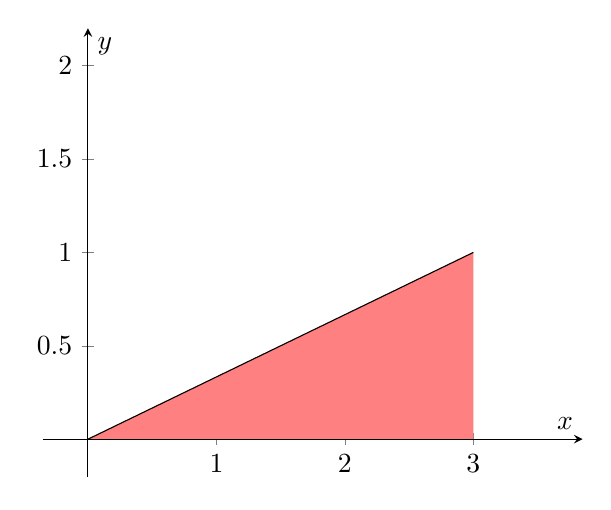
\begin{tikzpicture}
    \begin{axis}[axis lines=middle,
                 xlabel=\(x\), ylabel=\(y\),
                 ymin=0, ymax=2,
                 xmin=0, xmax=3.5,
                 enlargelimits]
      \addplot[name path=F, domain={0:3}]{x/3};
      \addplot[name path=G, domain={0:3}]{0};
      \addplot[color=red!50] fill between [
               of=F and G, soft clip={domain=0:3}];
    \end{axis}
  \end{tikzpicture}
\end{center}
\begin{align*}
  \int_{0}^{1}\int_{3y}^{3}\e^{x^2}\diff{x}\diff{y} &=
    \int_{0}^{3}\int_{0}^{\frac{x}{3}}\e^{x^2}\diff{y}\diff{x} \\
  &= \int_{0}^{3}\e^{x^2}\bigg[y\bigg]_{0}^{\frac{x}{3}}\diff{x} \\
  &= \frac{1}{3}\int_{0}^{3}x\e^{x^2}\diff{x} \\
  &= \frac{1}{6}\int_{0}^{3}2x\e^{x^2}\diff{x} \\
  &= \frac{1}{6}\bigg[\e^{x^2}\bigg]_{0}^{3} \\
  &= \frac{1}{6}(\e^9-\e^0) \\
  &= \frac{\e^9-1}{6}
\end{align*}

\subsubsection*{Exercise 53​}
Evaluate the integral by reversing the order of integration.
\[ \int_{0}^{1}\int_{\sqrt{x}}^{1}\sqrt{y^3+1}\diff{y}\diff{x} \]
\begin{center}
  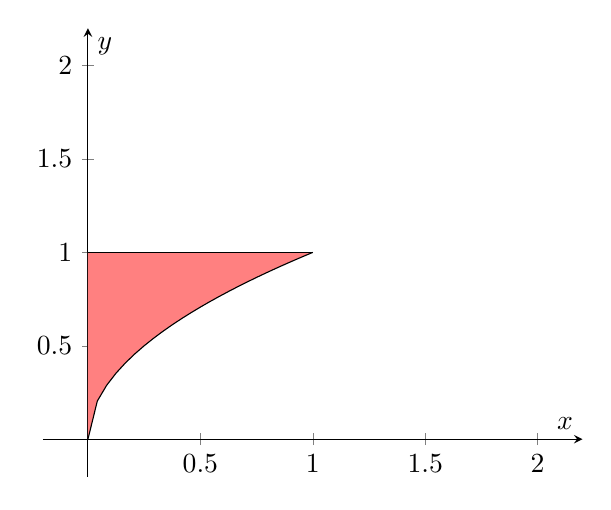
\begin{tikzpicture}
    \begin{axis}[axis lines=middle,
                 xlabel=\(x\), ylabel=\(y\),
                 ymin=0, ymax=2,
                 xmin=0, xmax=2,
                 enlargelimits]
      \addplot[name path=F, domain={0:1}]{sqrt(x)};
      \addplot[name path=G, domain={0:1}]{1};
      \addplot[color=red!50] fill between [
               of=F and G, soft clip={domain=0:1}];
    \end{axis}
  \end{tikzpicture}
\end{center}
\begin{align*}
  \int_{0}^{1}\int_{\sqrt{x}}^{1}\sqrt{y^3+1}\diff{y}\diff{x} &=
    \int_{0}^{1}\int_{0}^{y^2}\sqrt{y^3+1}\diff{x}\diff{y} \\
  &= \int_{0}^{1}\sqrt{y^3+1}\bigg[x\bigg]_{0}^{y^2}\diff{y} \\
  &= \frac{1}{3}\int_{0}^{1}3y^2\sqrt{y^3+1}\diff{y} \\
  &= \frac{1}{3}\bigg[\frac{2}{3}(y^3+1)^{\frac{3}{2}}\bigg]_{0}^{1}\diff{y} \\
  &= \frac{2}{9}(2^{\frac{3}{2}}-1^{\frac{3}{2}}) \\
  &= \frac{2(2\sqrt{2}-1)}{9} \\
  &= \frac{4\sqrt{2}-2}{9}
\end{align*}

\begin{center}
  If you have any questions, comments, or concerns, please contact me at
  alvin@omgimanerd.tech
\end{center}

\end{document}
